\providecommand{\main}{../../../..}
\documentclass[\main/dresen_thesis.tex]{subfiles}
\begin{document}
  \label{sec:colloidalCrystals:layers:gisaxs}
  \begin{figure}[tb]
    \centering
    \includegraphics{colloidalCrystals_GISAXS_SVcbar}
    \includegraphics{colloidalCrystals_GISAXS_CC-Fe-0_37_lowerAngle}
    \includegraphics{colloidalCrystals_GISAXS_CC-Fe-0_37_withPeaks}
    \caption{\label{fig:colloidalCrystals:layers:gisaxs}GISAXS data of CC-Fe-0.37 measured under an incident angle of $0.155 ^\circ$ (left) and $0.205 ^\circ$ (right). Additionally marked in the right plot are the calculated reflection positions for an orthorhombic unit cell with $a \eq 16.6 \unit{nm}$, $b \eq 33.9 \unit{nm}$ and $c \eq 51.3 \unit{nm}$ and the in the text discussed selection rules.}
  \end{figure}

  To determine the superstructure of the nanocubes in the colloidal crystal, grazing-incidence small X-ray scattering is performed on the selected sample CC-Fe-0.37 at the GALAXI instrument (\refsec{ch:lss:galaxi}).
  The obtained detector images for the two incident angles $\alpha_i \eq 0.155^\circ$ and $\alpha_i \eq 0.205^\circ$ are shown in \reffig{fig:colloidalCrystals:layers:gisaxs}.
  The data shows the emergence of multiple broad reflections on top of additionally weakly visible form factor rings.

  The extended width of the reflections and the elongation of the reflection along $q_z$ indicates to a relatively thin layer structure of only few unit cells for the vertical direction in CC-Fe-0.37.
  Also the visibility of rings can be interpret that the nanocubes are measured in varied rotational orientation in the sample.

  The reflection positions are estimated manually from the GISAXS measured at $\alpha_i \eq 0.205 ^\circ$ and tabulated in \reftab{tab:colloidalCrystals:gisaxs:reflections}.
  Using an orthorhombic unit cell, the reflections are indexed, where with $a \eq 16.6(2) \unit{nm}$, $b \eq 33.9(3) \unit{nm}$ the $q_y$ positions of the reflections is closely reproduced for most points, from which the series (02l), (11l), (13l), (20l), (22l) and (06l) are determined.
  By variation of $c$, a value of $c \eq 51.3(5) \unit{nm}$ is determined to reproduce most $q_z$ positions, where for (02l), (22l) and (06l) the extinction rules $l \eq 4n + 2$, for (11l) and (13l) $l \eq 2n + 1$ and for (20l) $l \eq 4n$ are observed.
  The final lattice constants and the error estimate have been obtained by minimizing the $\chi^2$ distance between the manually determined peak positions and the calculated positions of the associated indices.
  The errors are approximated graphically from the lattice constant values for which the $\chi^2$ distance changes by a value of $1$ as described in \cite{Bevington_2003_Datar}.

  \begin{table}[!htbp]
    \centering
    \caption{\label{tab:colloidalCrystals:gisaxs:reflections}Determined reflection positions from \reffig{fig:colloidalCrystals:layers:gisaxs}, the closest index (hkl) in an orthorhombic unit cell with lattice constants of $a \eq 16.6(2) \unit{nm}$, $b \eq 33.9(3) \unit{nm}$, $c \eq 51.3(5) \unit{nm}$ and the thereby calculated theoretical position $q^{hkl}_y$ and $q^{hkl}_z$. The $\pm$ sign on the index indicates the positive or negative sign in \refeq{eq:colloidalCrystals:layerChar:gisaxs:reflexPosition}.}
    \begin{tabular}{ c | c | l | c | c}
      $q_y\,/ \unit{nm^{-1}}$ & $q_z\, / \unit{nm^{-1}}$ & (hkl) & $q^{hkl}_y\,/ \unit{nm^{-1}}$ & $q^{hkl}_z\,/ \unit{nm^{-1}}$\\
      \hline
      $0.38(1)$ & $0.33(3)$ & $(022)^{-}$ & $0.37$ & $0.36$\\
      $0.33(1)$ & $0.85(1)$ & $(026)^{-}$ & $0.37$ & $0.81$\\
      $0.44(1)$ & $0.29(3)$ & $(111)^{-}$ & $0.42$ & $0.30$\\
      $0.45(2)$ & $0.82(2)$ & $(115)^{+}$ & $0.42$ & $0.90$\\
      $0.65(1)$ & $0.67(1)$ & $(135)^{-}$ & $0.67$ & $0.69$\\
      $0.76(2)$ & $0.55(2)$ & $(204)^{-}$ & $0.76$ & $0.57$\\
      $0.83(1)$ & $0.40(2)$ & $(222)^{-}$ & $0.84$ & $0.36$\\
      $0.86(3)$ & $1.03(3)$ & $(226)^{+}$ & $0.84$ & $1.02$\\
      $1.13(2)$ & $0.78(2)$ & $(066)^{-}$ & $1.11$ & $0.81$\\
      \hline
    \end{tabular}
  \end{table}

  \begin{figure}[tb]
    \centering
    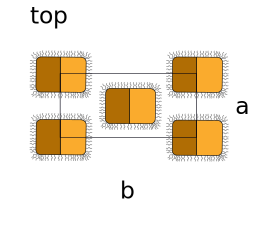
\includegraphics{colloidalCrystal_bctUnitCellTopView}
    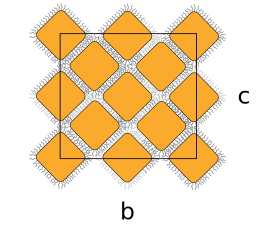
\includegraphics{colloidalCrystal_bctUnitCell}
    \caption{\label{fig:colloidalCrystals:layers:gisaxsBCTUCDepiction}Top view (left) and projection of the side view (right) on the $bct$ unit cell with [101] orientation reproduced as presented in \cite{Wetterskog_2016_Tunin}.}
  \end{figure}

  Inspecting the determined lattice constants, it is visible that $b/a \eq 2.04(3)$ and $c/a \eq \sqrt{9.6(3)}$.
  This can be compared to the structure evaluation of iron oxide mesocrystals in \cite{Wetterskog_2016_Tunin}, where a body-centered tetragonal $(bct)$ unit cell is used to index the observed reflection positions of the mesocrystals.
  In the study \cite{Wetterskog_2016_Tunin}, two orientations are observed, one with the [100] direction of the $bct$ unit cell parallel to the substrate normal and one with the [101] direction.
  For coherent grain boundaries of the two growth directions a ratio of $c/a \eq \sqrt{3}$ in a tetragonal unit cell ($a \eq b$) is derived.
  The [101] growth direction is described with an corresponding orthorhombic unit cell, which has $b \eq 2 a$ and $c \eq \sqrt{12} a$ as depicted in \reffig{fig:colloidalCrystals:layers:gisaxsBCTUCDepiction}.
  This is close to the ratios observed in the determined orthorhombic unit cell for the colloidal crystals.
  The $c$ constant is slightly smaller with $c \approx \sqrt{9.6(3)} a$, which indicates that not a perfect [101] orientation is observed.
  This is also in connection with SEM in \refsec{sec:colloidalCrystals:layers:sem}, where for CC-Fe-0.37 a tilt angle of $\approx 41(1) ^\circ$ is observed.
  For a [101] $bct$ structure with $c/a \eq \sqrt{12}$ and $b/a \eq 2$, an angle of $\arctan(\sqrt{12}/2) \eq 60 ^\circ$ or perpendicular to that $30^\circ$ would however be expected.

  The mesocrystal study by Wetterskog \etal \cite{Wetterskog_2016_Tunin} furthermore discusses the influence of the nanoparticle size.
  In the study, nanoparticles with a similar size as the discussed nanocubes, which have an edge length of $12.6(8) \unit{nm}$ and a superball exponent of $1.45$, show a preference for the [101] growth direction.
  This observation is in a close agreement with the observation made for the nanocubes in this colloidal crystal study, which have a size of $12.26(4) \unit{nm}$ and a superball exponent of $2.15(7)$, as determined from SAXS in \refsec{sec:colloidalCrystals:nanoparticle:sas}.

  According to the study, smaller nanocubes with a size of $9.6(4) \unit{nm}$ and a superball exponent of $1.9$ prefer the [001] growth direction instead for the $bct$ structure, and for larger nanocubes with a size of $13.6(8) \unit{nm}$ and a superball exponent of $1.85$ a transition to a simple cubic structure can be observed.
  Due to the strong parallels between the same sized nanocubes of the mesocrystal study and this colloidal crystal study, it might therefore be interesting in a future study to determine the effect of the nanocube size on the colloidal growth.
  In the mesocrystal study, magnetic fields are further used during the drying process to manipulate the structure formation, which has also not been attempted within this thesis and might be of interest in a future study.
\end{document}